%%%%%%%%%%%%%%%%%%%%%%%%%%%%%%%%%%%%%%%%%
% Focus Beamer Presentation
% LaTeX Template
% Version 1.0 (8/8/18)
%
% This template has been downloaded from:
% http://www.LaTeXTemplates.com
%
% Original author:
% Pasquale Africa (https://github.com/elauksap/focus-beamertheme) with modifications by 
% Vel (vel@LaTeXTemplates.com)
%
% Template license:
% GNU GPL v3.0 License
%
% Important note:
% The bibliography/references need to be compiled with bibtex.
%
%%%%%%%%%%%%%%%%%%%%%%%%%%%%%%%%%%%%%%%%%

%----------------------------------------------------------------------------------------
%	PACKAGES AND OTHER DOCUMENT CONFIGURATIONS
%----------------------------------------------------------------------------------------

\documentclass[aspectratio=169]{beamer}

\usetheme{focus} % Use the Focus theme supplied with the template
% Add option [numbering=none] to disable the footer progress bar
% Add option [numbering=fullbar] to show the footer progress bar as always full with a slide count

% Uncomment to enable the ice-blue theme
%\definecolor{main}{RGB}{92, 138, 168}
%\definecolor{background}{RGB}{240, 247, 255}

%------------------------------------------------

\usepackage{booktabs} % Required for better table rules

%----------------------------------------------------------------------------------------
%	 TITLE SLIDE
%----------------------------------------------------------------------------------------

\title{Nonnegative Matrix Factorization }

\subtitle{Analysing Fruit Spectograms}

\author{Christoph Lange}

\titlegraphic{
\includegraphics[scale=0.25]{images/strawberry.png}} % Optional title page image, comment this line to remove it
% Thanks cleanpng for the picture : https://www.cleanpng.com/png-strawberry-shortcake-clip-art-cartoon-strawberry-198600/
%\institute{Institute Name \\ Institute Address}

\date{\today}

%------------------------------------------------

\begin{document}

%------------------------------------------------

\begin{frame}
	\maketitle % Automatically created using the information in the commands above

\end{frame}

%----------------------------------------------------------------------------------------
%	 SECTION 1
%----------------------------------------------------------------------------------------

\section{Fruit Spectrogram  \\ Approximation} % Section title slide, unnumbered

%------------------------------------------------

\begin{frame}{Fruit Puree Spectrograms}
	\begin{columns}
		\column{0.35\textwidth}
		Fruit puree  \href{https://data.mendeley.com/datasets/frrv2yd9rg/1}{\color{brown}{dataset}} contains
			 \begin{itemize}
				\item  $N = 983$ fruit spectrograms 
				\item $p = 235$ frequencies per spectrogram
				\item labels "Strawberry" or "NON-Strawberry"
			\end{itemize}
		
		\column{0.65\textwidth}
			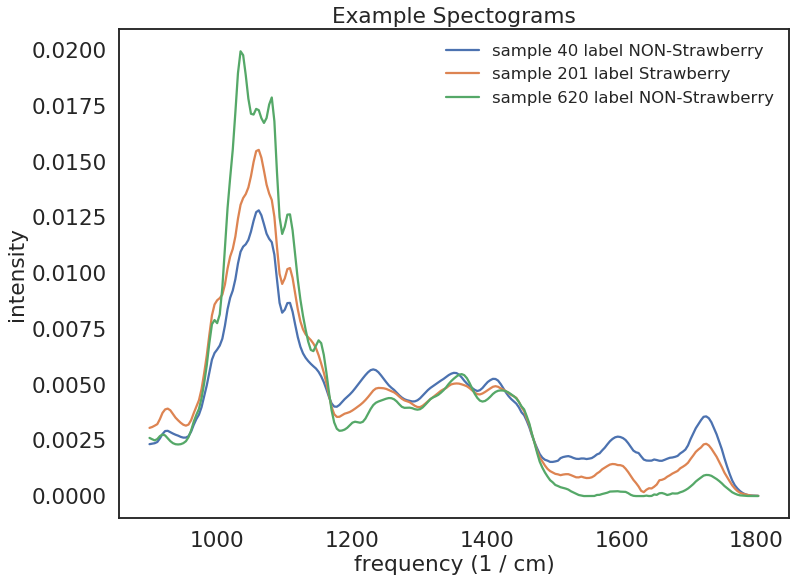
\includegraphics[width=\linewidth]{images/three_examples.png}
	\end{columns}

\end{frame}

%------------------------------------------------

\begin{frame}{Nonnegative Matrix Factorization}

We represent $n$ spectrograms by
\begin{equation*}
X \in \mathbb{R}^{n x p}  \quad x_{i j} \geq 0
\end{equation*}
with one row $x_i$ being one spectrogram and approximate them.
\begin{equation*}
X \approx W \cdot H    \qquad  W \in \mathbb{R}^{n \times r}, H \in \mathbb{R}^{r \times p} \quad w_{i j} \geq 0 , h_{i j} \geq 0
\end{equation*}
Remarks:
\begin{itemize}
\item each row  $x_i = (x_{i 1}, x_{i 2}, \dots , x_{i p} ) $ is one spectogram
\item rows of H, $h_i = (h_{i, 1}, \dots , h_{i, p})   \quad i \in \{1, \dots , r \}$, form an $r$ dimensional basis
\item rows of W, $w_i = (w_{i 1}, \dots , w_{i r} )$ are the coordinates
\item $x_i \approx \sum_{j=1}^{r} w_{i j } h_{j} $ 
\item $(W \cdot H)^T = H^T \cdot W^T $, i.e. we can swap the roles of $W$ and $H$
\end{itemize}
\end{frame}

%------------------------------------------------

\begin{frame}{Example Factorization}

	\begin{columns}
		\column{0.35\textwidth}
			Steps
			 \begin{itemize}
				\item choose $r=4 $ dimensions
				\item find $W$ and $H$ such that $X \approx W \cdot H$ for  training set
				\item plot $\{ h_1, h_2, h_3, h_4 \} $
			\end{itemize}
		
		\column{0.65\textwidth}
			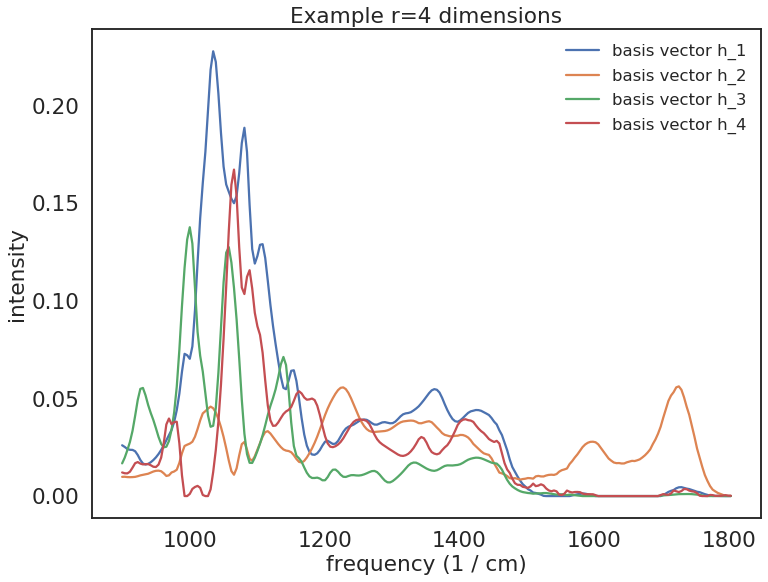
\includegraphics[width=\linewidth]{images/four_basis_vectors.png}
	\end{columns}
\end{frame}

%------------------------------------------------

\begin{frame}{Example Factorization}

	\begin{columns}
		\column{0.35\textwidth}
			Pick one spectrogram $x_i$ and compare
			\begin{equation*}
			x_i \approx \sum_{j=1}^{r} w_{i j } h_{j} = w_i \cdot H
			\end{equation*}
			The right hand side is the i-th row of $W \cdot H$.
		\column{0.65\textwidth}
			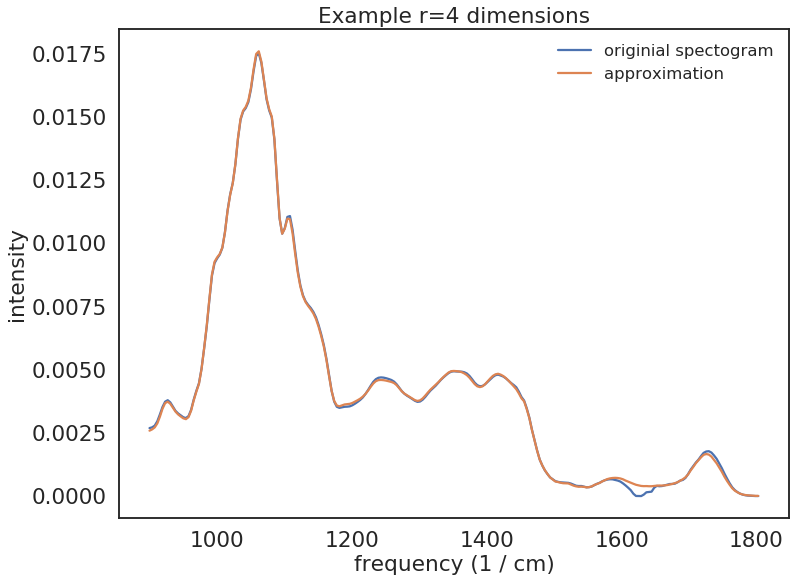
\includegraphics[width=\linewidth]{images/original_approx.png}
	\end{columns}
\end{frame}

%------------------------------------------------
\section{How does Nonnegative Matrix Factorization approximate?}

\begin{frame}{How does NMF approximate?}

Each spectrogram $x_i \in R^p$ should be close to it approximation $w_i H \in \mathbb{R}^p $  , i.e. the distance 
\begin{equation*}
d(x_i, w_i  H) = \left\lVert x_i - w_i  H \right\rVert 
\end{equation*}
between both should be small for all $ i  \in \{ 1, \dots , n \} $. Hence we minimize the sum of squared distances 
\begin{equation*}
\sum_{i = 1}^{n} \left\lVert x_i - w_i H\right\rVert^2  = \left\lVert X - W H\right\rVert^2_F
\end{equation*}
which is the Frobenius norm of both matricies.
\end{frame}

%------------------------------------------------
\begin{frame}{Minimization Problem}

	\begin{columns}
		\column{0.35\textwidth}
			Choose $r$ components and minimize 
			\begin{equation*}
			 \min_{ W, H }  \quad \left\lVert X - W H\right\rVert^2_F
			\end{equation*}
			How close is good enough?
		\column{0.65\textwidth}
			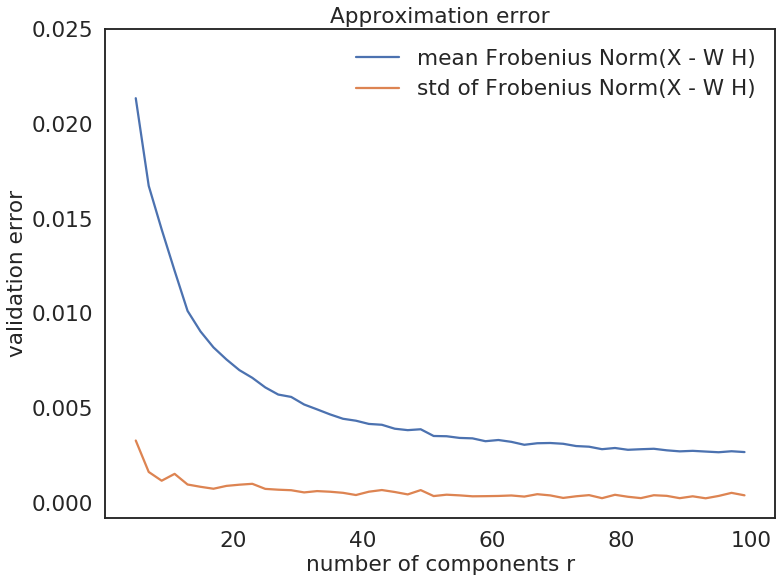
\includegraphics[width=\linewidth]{images/error_per_component.png}
	\end{columns}
\end{frame}

%------------------------------------------------

\begin{frame}{Use NMF for Strawberry Detection}

	\begin{columns}
		\column{0.35\textwidth}
			We do not want to minimize
			\begin{equation*}
			 \min_{ W, H }  \quad \left\lVert X - W H\right\rVert^2_F
			\end{equation*}
			but perform well on the classification task
			\begin{equation*}
			\min_{r}  - \sum_{i} \sum_{j =1}^{2}  y_i \log( \hat{y}_i) 
			\end{equation*}			
			$r=21$ might be optimal, but we choose $r=15$ for illustrative purposes.
		\column{0.65\textwidth}
			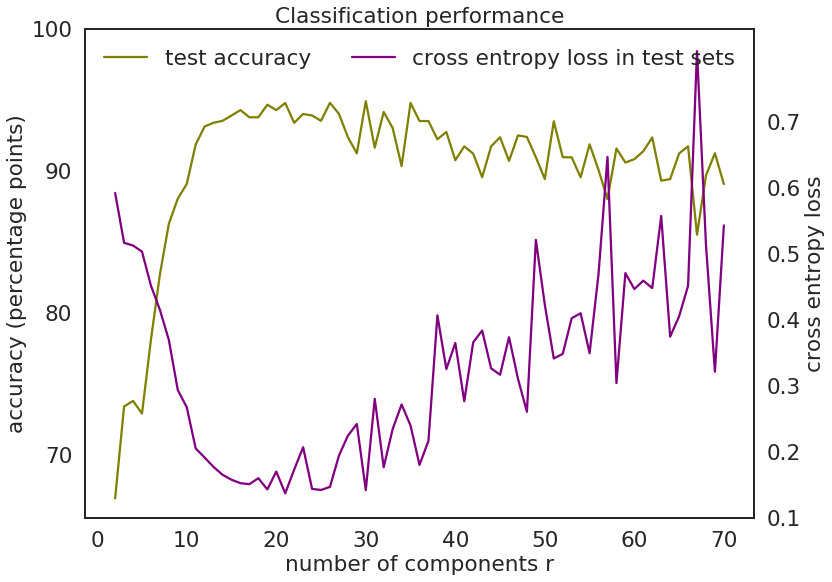
\includegraphics[width=\linewidth]{images/fruit_accuracies.png}
	\end{columns}
\end{frame}
%------------------------------------------------

\begin{frame}{Strawberry Basis Vectors}

	\begin{columns}
		\column{0.35\textwidth}
		Take a look at all basis vectors $h_i$ where the model thinks 
		\begin{equation*}
		\hat{y}(e_i) > 1 - \hat{y}(e_i)
		\end{equation*}
		$h_i$ is a Strawberry.
		\begin{itemize}
		\item spectrograms $h_i$ capture distinct characteristica
		\item many frequencies $h_{i j} = 0$
		\end{itemize}

		\column{0.65\textwidth}
			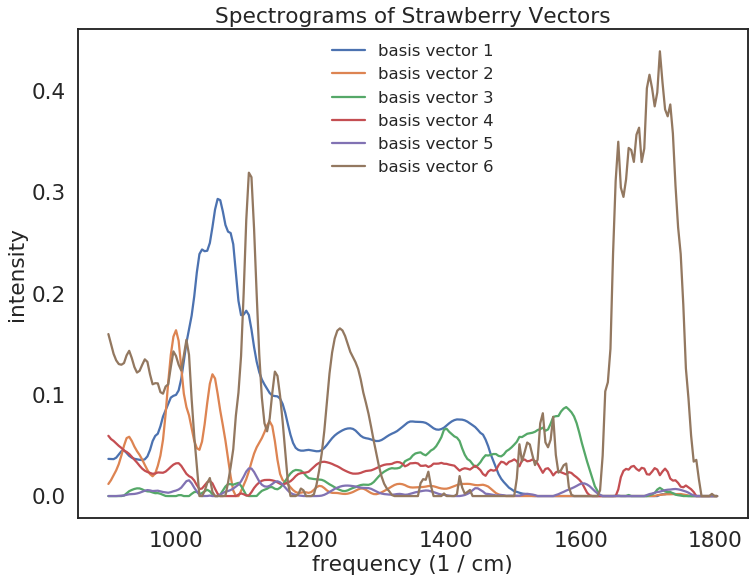
\includegraphics[width=\linewidth]{images/strawberry_basis_vectors.png}
	\end{columns}
\end{frame}

%------------------------------------------------
\begin{frame}{Properties of NMF}
	\begin{columns}[t]

	\column{0.55 \textwidth}
	\textbf{advantages}
	\begin{itemize}
	\item filters noise $X - W H $
	\item basis vectors $h_i$ capture joint phenomena
	\item basis vectors $h_i$ can be interpreted to draw conclusions about the dataset
	\item imposing $W W^T  = I $ makes NMF equivalent to K-means clustering
	\end{itemize}
	\column{0.45 \textwidth}
	\textbf{disadvantages}
	\begin{itemize}
	\item Finding coordinates $W$ requires solving $\min_{ W, H }  \quad \left\lVert X - W H\right\rVert^2_F$.
	\item limited to nonnegative matricies
	\end{itemize}
	\end{columns}
\end{frame}


%------------------------------------------------

\begin{frame}[focus]
	Thank you \\
	Questions?
\end{frame}

%----------------------------------------------------------------------------------------
%	 CLOSING/SUPPLEMENTARY SLIDES
%----------------------------------------------------------------------------------------

\appendix

\begin{frame}{References}
	\nocite{*} % Display all references regardless of if they were cited
	\bibliography{NMF_papers}
	\bibliographystyle{plain}
\end{frame}

%------------------------------------------------

\begin{frame}{NON Strawberry Basis Vectors}

	\begin{columns}
		\column{0.35\textwidth}

		\column{0.65\textwidth}
			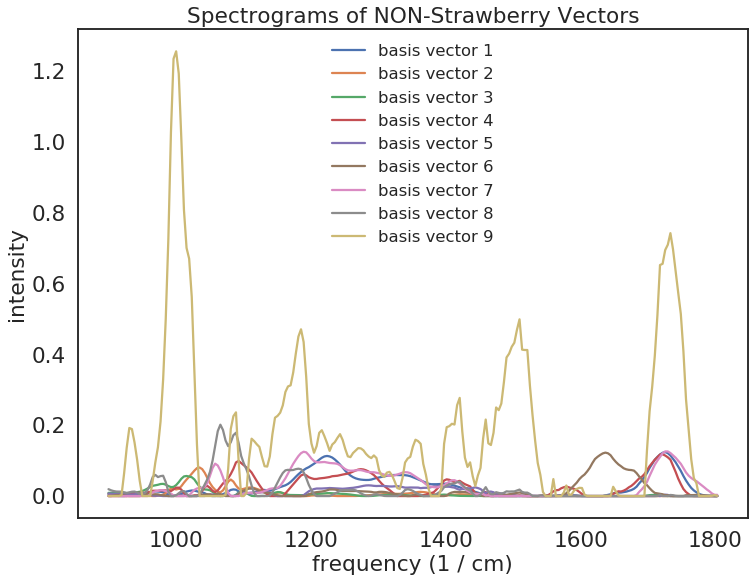
\includegraphics[width=\linewidth]{images/non_strawberry_basis_vectors.png}
	\end{columns}
\end{frame}

%------------------------------------------------

\begin{frame}{Bayesian Approach}
	The NMF solution $W, H$ that minimizes
	\begin{equation*}
	 \quad \left\lVert X - W H\right\rVert^2_F
	\end{equation*}
	is the maximum likelihood estimator assuming Gaussian noise
	\begin{equation*}
	X \sim N( W H, \sigma^2)
	\end{equation*}
	Bayesian approach enables 
	\begin{equation*}
	P(W, H \mid X) \propto  P(X \mid W, H ) P(W, H)
	\end{equation*}
	incorporating domain knowledge about $P(H) $.
\end{frame}
%------------------------------------------------
\end{document}
